\section{Diskussion}
\label{sec:Diskussion}
Insgesamt lässt sich erkennen, dass die gemessenen Positionen und Dicken für die größeren Störstellen einen
geringeren Fehler aufweisen als die kleineren Störstellen. Dies lässt sich durch das Auflösungsvermögen
erklären, dass bei niederigeren Frequenzen bzw. größeren Wellenlängen kleiner ist. Da aber bei kleineren
Wellenlängen die gemessenen Amplituden stärker abfallen, muss einer Ultraschallsonde gewählt werden, die
das Auflösungsvermögen maximiert und dabei die Amplituden noch groß genug lässt. Weiterhin haben sich B-Scans
mit zwar gut erkennbaren Störstellen ergeben, dennoch sind die Messwerte für die Störstellen und Dicken wesentlich
schlechter als die des A-Scans. Hierbei lässt sich das Verschmieren wieder über das Auflösungsvermögen
erklären. Für den B-Scan des Brustmodels ließen sich beide ertasteten Tumore verifizieren und sie weisen eine
realistische Dicke auf.

\addsec{Anhang}
\label{sec:Anhang}
\begin{figure}
    \centering
    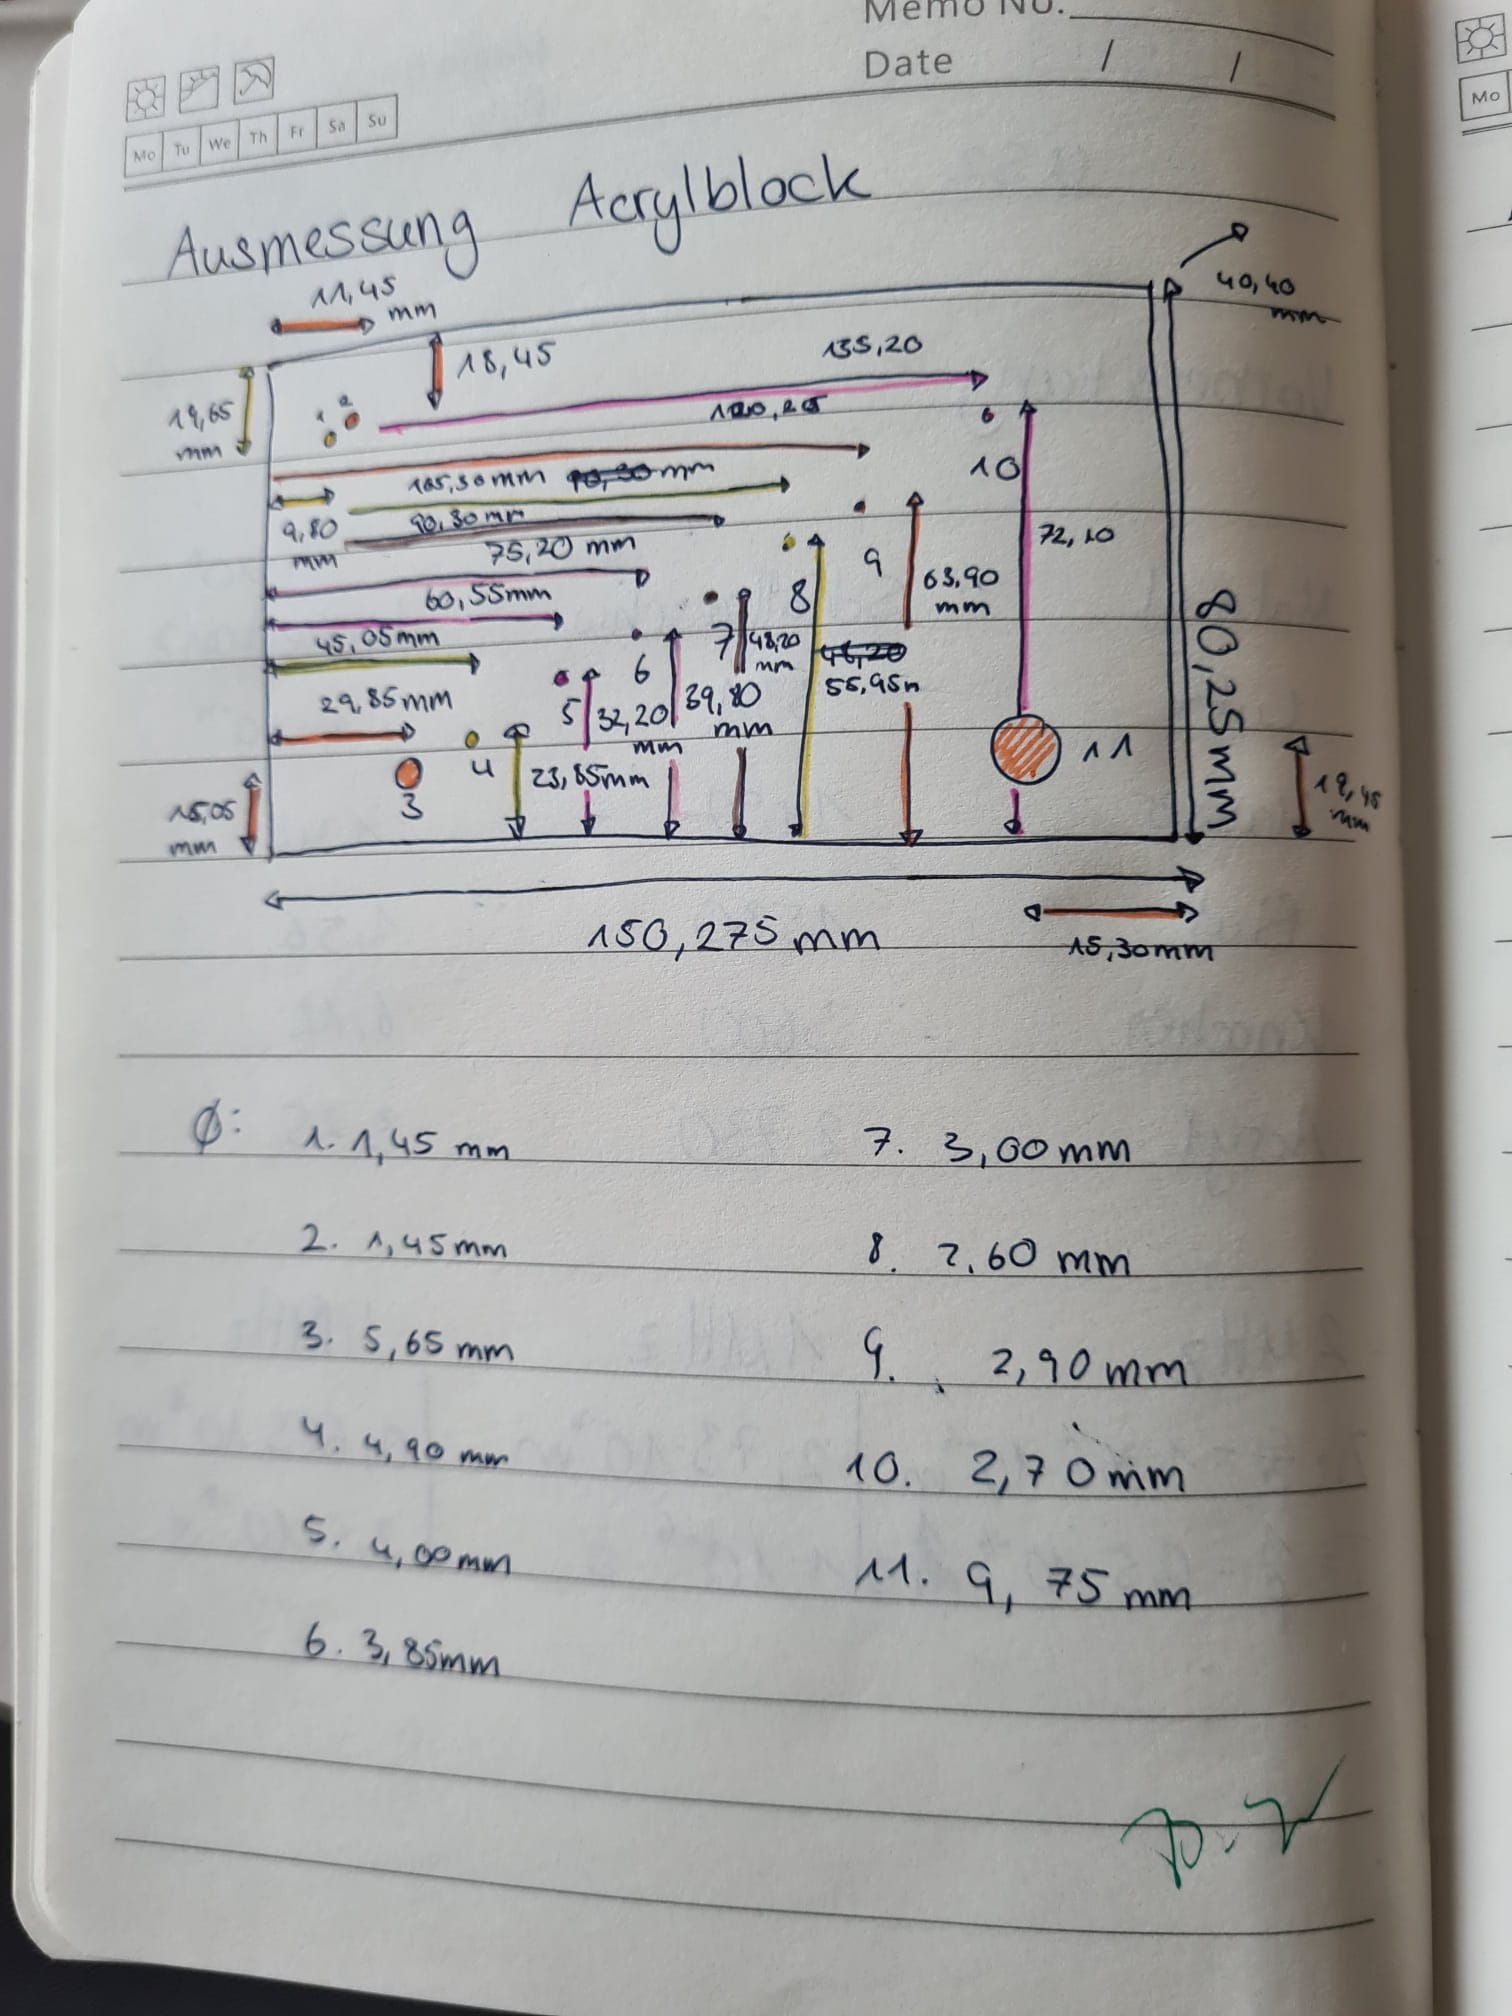
\includegraphics[width=0.7\textwidth]{messwerte/index.jpg}
    \caption{Abmessungen des Acrylblocks.}
\end{figure}

\begin{figure}
    \centering
    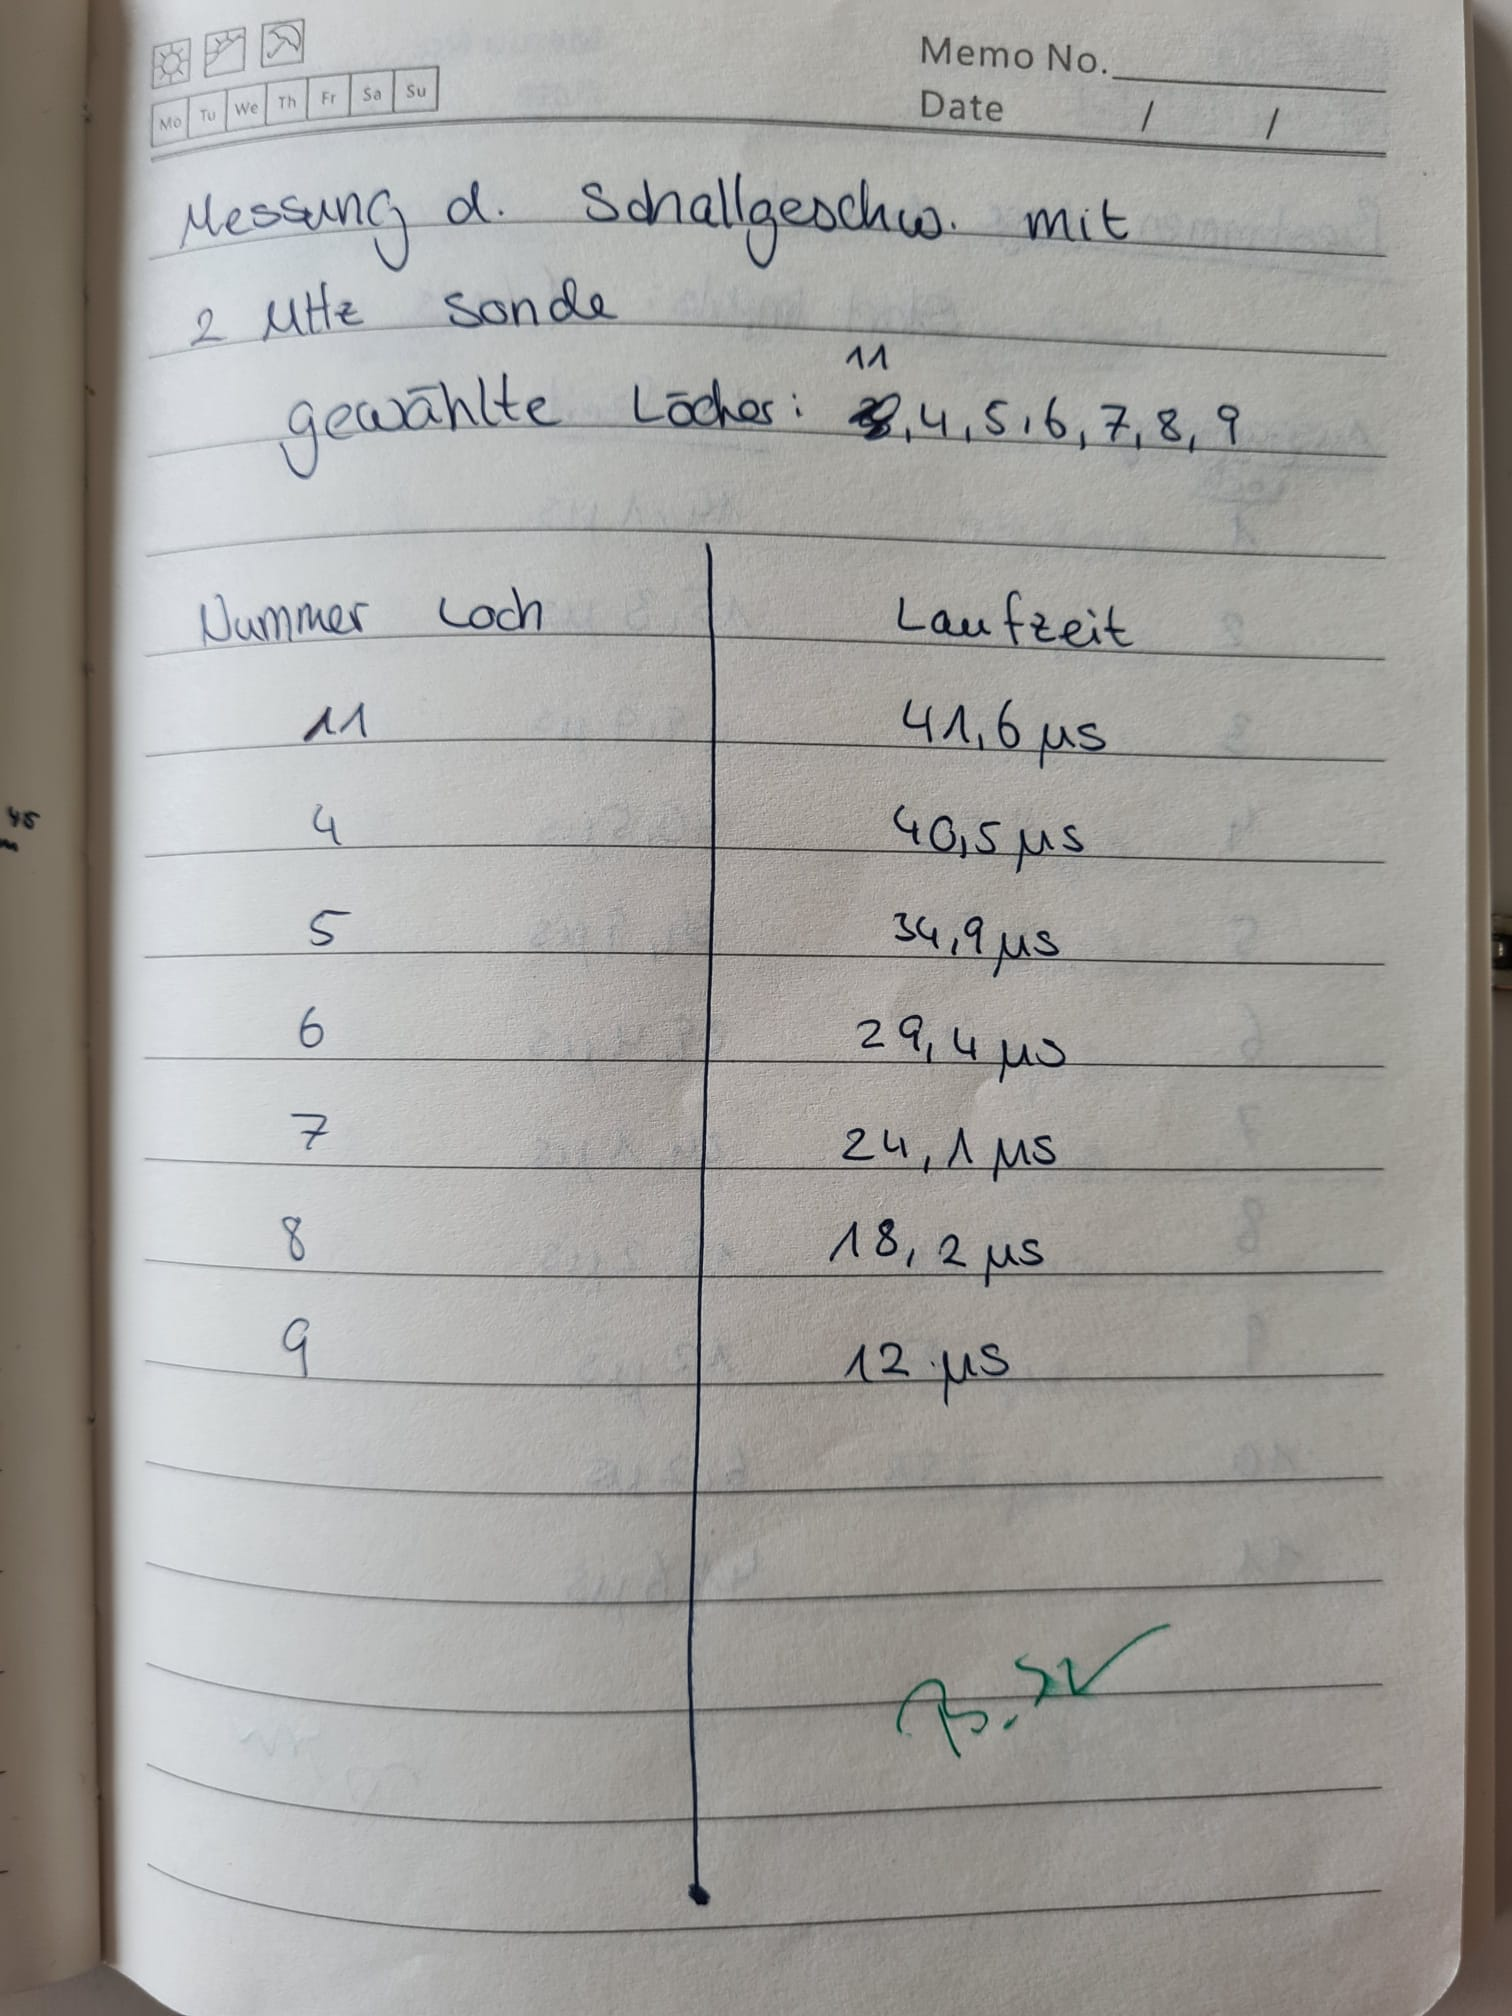
\includegraphics[width=0.7\textwidth]{messwerte/index2.jpg}
    \caption{Messung der Schallgeschwindigkeit mit $2\,\unit{\mega\hertz}$-Sonde.}
\end{figure}

\begin{figure}
    \centering
    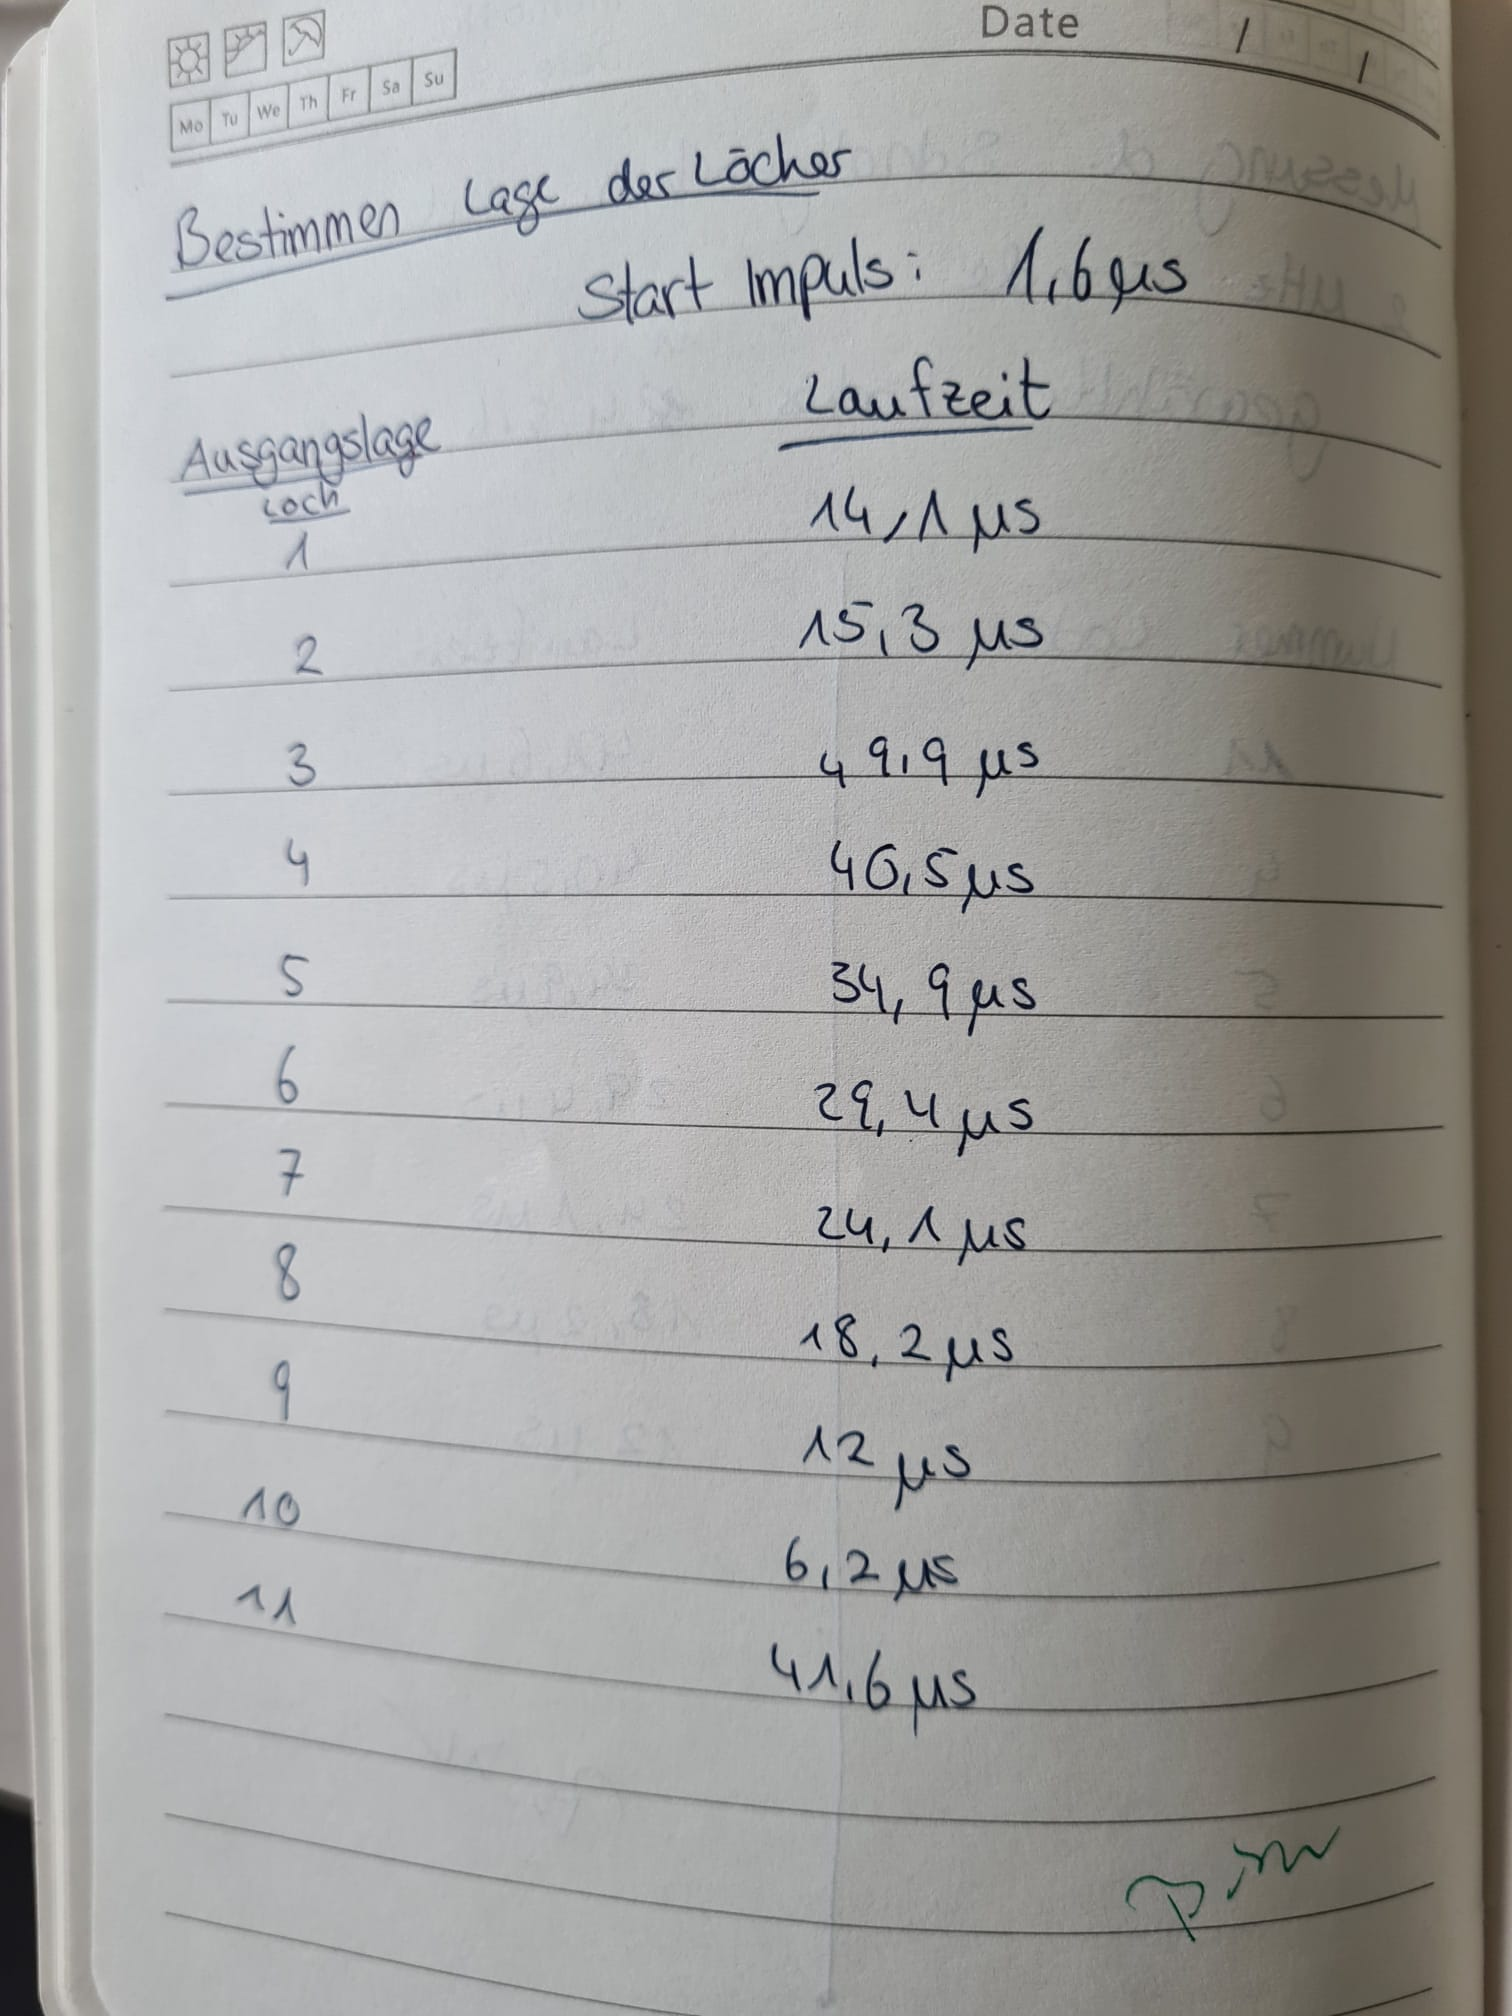
\includegraphics[width=0.7\textwidth]{messwerte/index3.jpg}
    \caption{Lage Bestimmung der Löcher im Acrylblock.}
\end{figure}

\begin{figure}
    \centering
    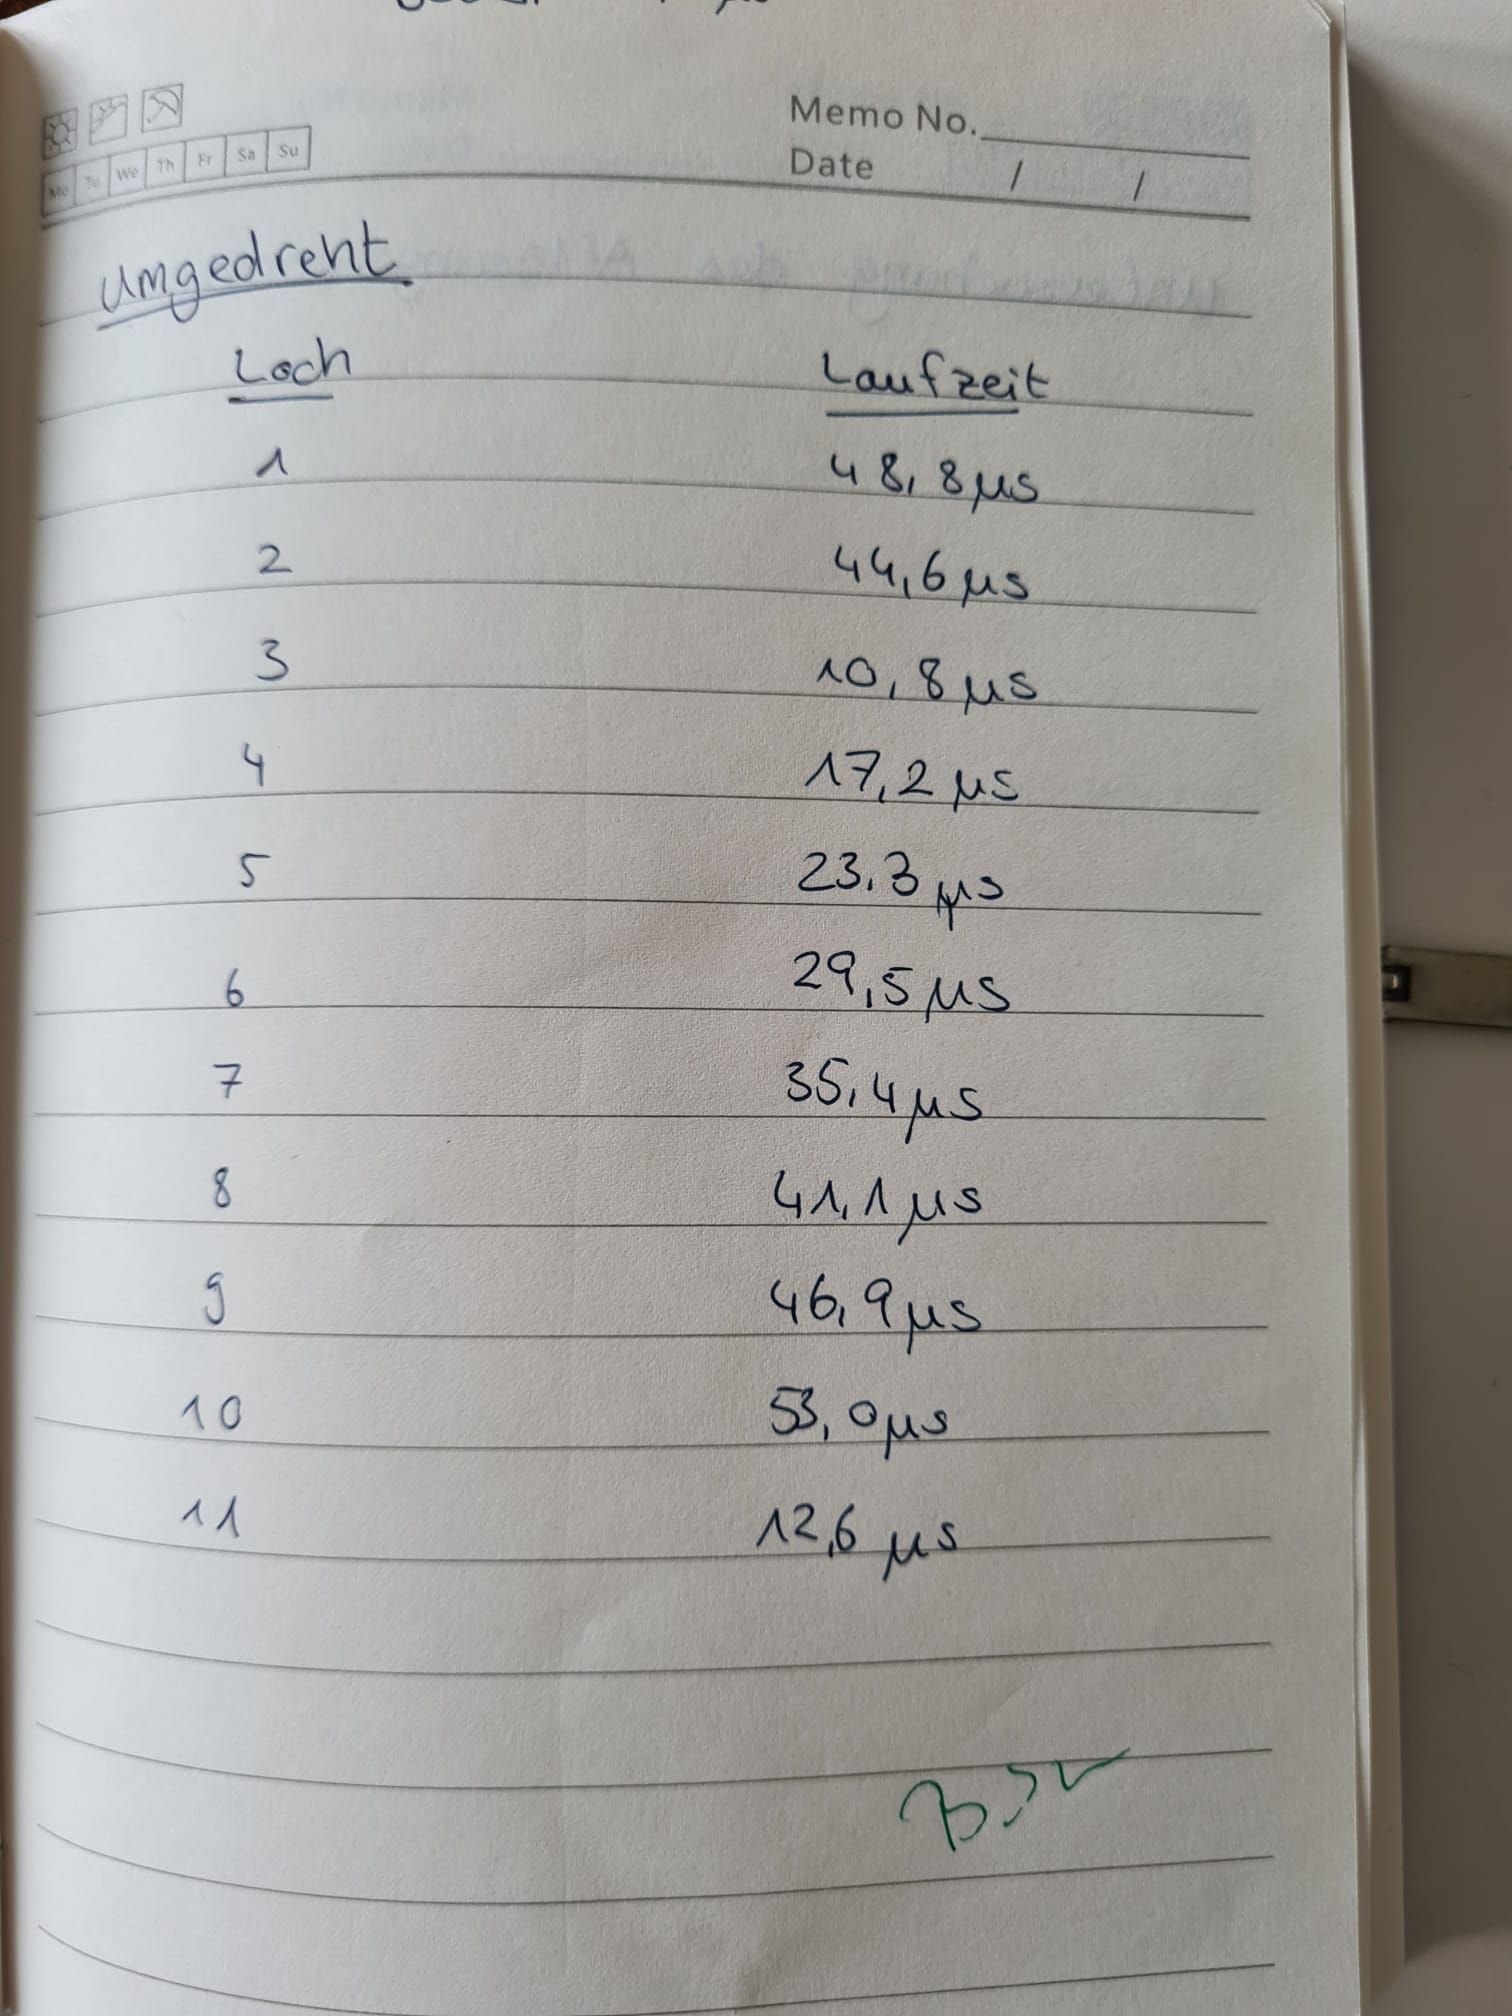
\includegraphics[width=0.7\textwidth]{messwerte/index4.jpg}
    \caption{Lage Bestimmung der Löcher im Acrylblock im umgedrehten Zustand.}
\end{figure}